We sample functions from a multivariate normal distribution with an RBF kernel and a randomly chosen length scale. The functions are defined on a grid of 128 points in the interval $[0,1]$. From these 128 points, a subset of 5 to 50 points is chosen randomly to be the set of context points. This subset is the input data from which the underlying function must be estimated. Our train datasets consist of 100.000 functions and test-datasets consist of 1000 functions. The test datasets have fixed subset sizes (\autoref{tab:fun_subset}). We generate two versions of all datasets. In both versions the RBF-Scale values for each sampled function are drawn from a beta-distribution. Version-A uses parameters $\alpha = 2, \beta = 10$ and Version-B uses $\alpha = 2, \beta = 5$ (\autoref{tab:rbf_scale}). In total, we generate two training datasets and eight test datasets. \autoref{fig:beta_scales} shows the distribution from which the RBF-Scale values are drawn in Version-A and Version-B. The lower the RBF-Scale, the stronger the sampled functions vary in a given time frame. We can see this exemplary in \autoref{fig:gaussian}, where the most right function with RBF-Scale of $0.05$ varies much more than the left most function with RBF-Scale $0.27$. Therefore, Version-A Datasets contain more strongly varying functions and we consider it more difficult than Version-B.

\begin{table}[]
	\centering
	\caption{Number of functions and context point subset size for training and test datasets. The number of context points for the training datasets vary, while for test datasets they are fixed.}
	\begin{tabular}{c c c c c c}
		\toprule
		& Train & \multicolumn{4}{c}{Test}\\
		\midrule
		Functions & 100K & \multicolumn{4}{c}{1K}\\
		Subset size & 5-50 & 5 & 10 & 50 & 100  \\\bottomrule
	\end{tabular}
	\label{tab:fun_subset}
\end{table}

\begin{table}[]
	\centering
	\caption{Beta distribution parameters and resulting mean for the sampled RBF-Scale values for both dataset versions.}
	\begin{tabular}{c c c}
		\toprule
		& Version-A & Version-B\\
		\midrule
		Alpha & 2 & 2\\
		Beta & 10 & 5  \\\midrule
		Scale Mean & 0.15 & 0.3\\\bottomrule
	\end{tabular}
	\label{tab:rbf_scale}
\end{table}


\begin{figure}
	\centering
	\resizebox{0.4\textwidth}{!}{
		% This file was created with matplot2tikz v0.4.0.
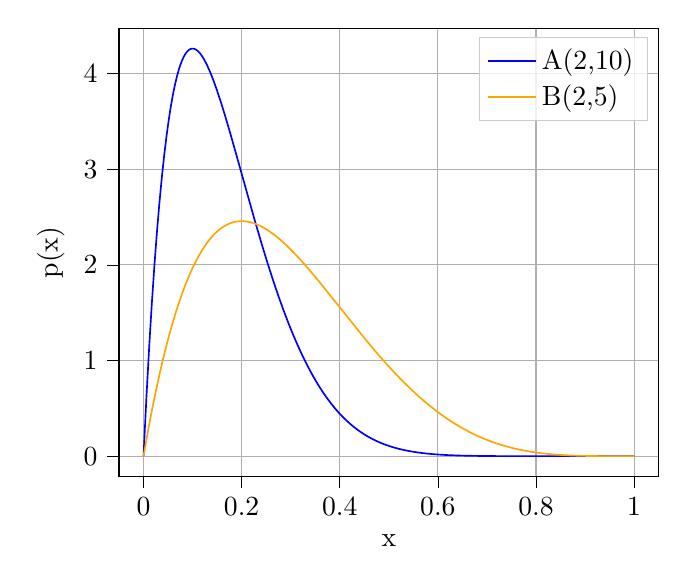
\begin{tikzpicture}

\definecolor{darkgray176}{RGB}{176,176,176}
\definecolor{lightgray204}{RGB}{204,204,204}
\definecolor{orange}{RGB}{255,165,0}

\begin{axis}[
legend cell align={left},
legend style={fill opacity=0.8, draw opacity=1, text opacity=1, draw=lightgray204},
tick align=outside,
tick pos=left,
x grid style={darkgray176},
xlabel={x},
xmajorgrids,
xmin=-0.05, xmax=1.05,
xtick style={color=black},
y grid style={darkgray176},
ylabel={p(x)},
ymajorgrids,
ymin=-0.213081150404745, ymax=4.47470415849965,
ytick style={color=black}
]
\addplot [semithick, blue]
table {%
0 0
0.00600600242614746 0.625795364379883
0.0120120048522949 1.18515026569366
0.0170170068740845 1.60394740104675
0.022022008895874 1.9824925661087
0.0270270109176636 2.32326078414917
0.0320320129394531 2.62860941886902
0.0370370149612427 2.90078258514404
0.0420420169830322 3.14191579818726
0.0470470190048218 3.35403966903687
0.0520520210266113 3.53908467292786
0.056056022644043 3.66885948181152
0.0600600242614746 3.78337502479553
0.0640640258789062 3.88349080085754
0.0680680274963379 3.97003054618835
0.0720720291137695 4.04378366470337
0.0760760307312012 4.10550594329834
0.0790790319442749 4.1443395614624
0.0820820331573486 4.17710781097412
0.0850850343704224 4.20409488677979
0.0880880355834961 4.22557544708252
0.0910910367965698 4.24181604385376
0.0930930376052856 4.24985885620117
0.095095157623291 4.25576162338257
0.0970971584320068 4.25959587097168
0.0980980396270752 4.2607593536377
0.0990991592407227 4.26143217086792
0.100100040435791 4.2616229057312
0.101101160049438 4.26134014129639
0.102102041244507 4.26059198379517
0.103103160858154 4.25938701629639
0.10510516166687 4.25563907623291
0.107107162475586 4.250159740448
0.109109163284302 4.24301290512085
0.112112164497375 4.22929906845093
0.115115165710449 4.21217155456543
0.118118166923523 4.19182348251343
0.122122168540955 4.16000604629517
0.126126170158386 4.12322044372559
0.131131172180176 4.07086420059204
0.136136174201965 4.01211977005005
0.142142176628113 3.93417382240295
0.149149179458618 3.83437347412109
0.157157182693481 3.71061825752258
0.166166186332703 3.56164717674255
0.17717719078064 3.36943769454956
0.193193197250366 3.07829689979553
0.227227210998535 2.45651459693909
0.241241216659546 2.21196222305298
0.253253221511841 2.01144313812256
0.264264225959778 1.8362330198288
0.275275230407715 1.67000436782837
0.285285234451294 1.52709674835205
0.295295238494873 1.39223885536194
0.305305242538452 1.26553130149841
0.314314365386963 1.15846419334412
0.323323249816895 1.0579389333725
0.332332372665405 0.963847637176514
0.341341376304626 0.876042604446411
0.350350379943848 0.794342994689941
0.358358383178711 0.726679801940918
0.366366386413574 0.663517355918884
0.374374389648438 0.604685544967651
0.382382392883301 0.55000627040863
0.390390396118164 0.499295949935913
0.398398399353027 0.452367186546326
0.406406402587891 0.409030914306641
0.414414405822754 0.369097352027893
0.422422409057617 0.332378268241882
0.429429411888123 0.302739262580872
0.436436414718628 0.275295972824097
0.443443417549133 0.249927878379822
0.450450420379639 0.22651731967926
0.457457423210144 0.204949855804443
0.464464426040649 0.18511426448822
0.471471428871155 0.166902899742126
0.47847843170166 0.150212168693542
0.485485553741455 0.134942173957825
0.492492437362671 0.120996952056885
0.499499559402466 0.108285069465637
0.506506443023682 0.0967187881469727
0.513513565063477 0.0862147808074951
0.520520448684692 0.0766938924789429
0.527527570724487 0.0680810213088989
0.534534454345703 0.0603053569793701
0.541541576385498 0.0532996654510498
0.549549579620361 0.0461554527282715
0.557557582855225 0.0398467779159546
0.565565586090088 0.0342921018600464
0.573573589324951 0.0294157266616821
0.582582592964172 0.0246539115905762
0.591591596603394 0.0205715894699097
0.600600600242615 0.0170861482620239
0.610610604286194 0.013823390007019
0.621621608734131 0.0108706951141357
0.633633613586426 0.00828838348388672
0.646646618843079 0.00610864162445068
0.660660743713379 0.00433588027954102
0.676676750183105 0.00287413597106934
0.695695638656616 0.00171232223510742
0.719719648361206 0.000845074653625488
0.751751780509949 0.000296115875244141
0.804804801940918 3.63588333129883e-05
1 0
};
\addlegendentry{A(2,10)}
\addplot [semithick, orange]
table {%
0 0
0.00900900363922119 0.260661602020264
0.0170170068740845 0.476638078689575
0.0250250101089478 0.678374767303467
0.033033013343811 0.866395711898804
0.0410410165786743 1.04121327400208
0.0490490198135376 1.20332884788513
0.0570570230484009 1.35323202610016
0.0650650262832642 1.49140179157257
0.0720720291137695 1.6030433177948
0.0790790319442749 1.70636606216431
0.0860860347747803 1.80167055130005
0.0930930376052856 1.88925051689148
0.100100040435791 1.96939384937286
0.107107162475586 2.04238224029541
0.113113164901733 2.09945774078369
0.119119167327881 2.15164923667908
0.125125169754028 2.19912314414978
0.131131172180176 2.24204325675964
0.137137174606323 2.28057026863098
0.143143177032471 2.31486105918884
0.14814817905426 2.34031200408936
0.15315318107605 2.36301612854004
0.158158183097839 2.38305950164795
0.163163185119629 2.40052652359009
0.167167186737061 2.41270136833191
0.171171188354492 2.42332291603088
0.175175189971924 2.43243193626404
0.179179191589355 2.44006991386414
0.183183193206787 2.44627642631531
0.186186194419861 2.45001602172852
0.189189195632935 2.45298957824707
0.192192196846008 2.45521306991577
0.195195198059082 2.456702709198
0.198198199272156 2.45747470855713
0.201201200485229 2.45754480361938
0.204204201698303 2.45692849159241
0.207207202911377 2.45564103126526
0.210210204124451 2.45369815826416
0.213213205337524 2.45111441612244
0.216216206550598 2.44790530204773
0.22022020816803 2.44267868995667
0.224224209785461 2.4364001750946
0.228228211402893 2.42910432815552
0.233233213424683 2.41860437393188
0.238238215446472 2.40663027763367
0.243243217468262 2.39324569702148
0.249249219894409 2.37540793418884
0.255255222320557 2.35573124885559
0.262262225151062 2.33058547973633
0.269269227981567 2.30323123931885
0.277277231216431 2.26945924758911
0.285285234451294 2.23322010040283
0.294294357299805 2.18976545333862
0.304304361343384 2.1384871006012
0.315315246582031 2.07887697219849
0.327327370643616 2.01056742668152
0.341341376304626 1.92731082439423
0.357357382774353 1.82853019237518
0.378378391265869 1.69493091106415
0.45445442199707 1.20763492584229
0.472472429275513 1.09768640995026
0.488488435745239 1.00322246551514
0.503503561019897 0.917885541915894
0.517517566680908 0.841341972351074
0.531531572341919 0.76801860332489
0.544544458389282 0.702972412109375
0.557557582855225 0.640970587730408
0.56956958770752 0.58651602268219
0.581581592559814 0.534779906272888
0.592592597007751 0.489771127700806
0.603603601455688 0.447086811065674
0.614614605903625 0.406728982925415
0.625625610351562 0.368689060211182
0.635635614395142 0.336103558540344
0.645645618438721 0.305398225784302
0.6556556224823 0.276546955108643
0.665665626525879 0.249517679214478
0.675675630569458 0.224273324012756
0.684684753417969 0.203044891357422
0.6936936378479 0.183194637298584
0.702702760696411 0.164685964584351
0.711711645126343 0.147480130195618
0.720720767974854 0.131535530090332
0.729729652404785 0.116809010505676
0.738738775253296 0.103255271911621
0.747747659683228 0.0908273458480835
0.756756782531738 0.0794768333435059
0.764764785766602 0.0702519416809082
0.772772789001465 0.0618036985397339
0.780780792236328 0.054095983505249
0.789789795875549 0.0462645292282104
0.798798799514771 0.0392718315124512
0.807807803153992 0.0330653190612793
0.816816806793213 0.0275923013687134
0.825825810432434 0.0228005647659302
0.834834814071655 0.0186378955841064
0.844844818115234 0.0146880149841309
0.854854822158813 0.0113821029663086
0.864864826202393 0.00865256786346436
0.875875949859619 0.00623714923858643
0.887887954711914 0.00420808792114258
0.900900840759277 0.00260663032531738
0.915915966033936 0.0013735294342041
0.93293285369873 0.000566244125366211
0.954954981803894 0.000117897987365723
0.99499499797821 0
1 0
};
\addlegendentry{B(2,5)}
\end{axis}

\end{tikzpicture}

	}
	\caption{Beta distributions for Version-A and -B from which the RBF scale is sampled. We consider the datasets for Version-A to be more challenging, however it has to be considered, that there is a large overlap between the distributions.}
	\label{fig:beta_scales}
\end{figure}

The size $n$ of the context point subsets is sampled uniformly $n\sim \mathcal{U}(5,50)$ and the resulting distribution is used for both train datasets.  For the test datasets, $n$ is fixed. The subsets are sampled uniformly from all possible subsets of size $n$, with the original grid always being 128 points. To be more in line with real world observations we add noise to the context points. We draw the noise from $\mathcal{N}(0,\sigma)$ with the standard deviation $\sigma$, which itself is sampled from $\mathcal{N}(0,0.1)$.